%---------------------------------------------------------------------------%
%-                                                                         -%
%-                           LaTeX Template                                -%
%-                                                                         -%
%---------------------------------------------------------------------------%
%- Copyright (C) Huangrui Mo <huangrui.mo@gmail.com> 
%- This is free software: you can redistribute it and/or modify it
%- under the terms of the GNU General Public License as published by
%- the Free Software Foundation, either version 3 of the License, or
%- (at your option) any later version.
%---------------------------------------------------------------------------%
%->> Document class declaration
%---------------------------------------------------------------------------%
\documentclass[doublesided]{Style/ucasthesis}%
%- Multiple optional arguments:
%- [<singlesided|doublesided|printcopy>]% set one or two sided eprint or print
%- [draftversion]% show draft version information
%- [fontset=<fandol|...>]% specify font set to replace automatic detection
%- [scheme=plain]% thesis writing of international students
%- [standard options for ctex book class: draft|paper size|font size|...]%
%---------------------------------------------------------------------------%
%->> Document settings
%---------------------------------------------------------------------------%
\usepackage[authoryear,myhdr,list]{Style/artratex}% document settings
%- usage: \usepackage[option1,option2,...,optionN]{artratex}
%- Multiple optional arguments:
%- [bibtex|biber]% set bibliography processor and package
%- [<numbers|super|authoryear|alpha>]% set citation and reference style
%- <numbers>: textual: Jones [1]; parenthetical: [1]
%- <super>: textual: Jones superscript [1]; parenthetical: superscript [1]
%- <authoryear>: textual: Jones (1995); parenthetical: (Jones, 1995)
%- <alpha>: textual: not available; parenthetical: [Jon95]
%- [geometry]% reconfigure page layout via geometry package
%- [lscape]% provide landscape layout environment
%- [myhdr]% enable header and footer via fancyhdr package
%- [color]% provide color support via xcolor package
%- [background]% enable page background
%- [tikz]% provide complex diagrams via tikz package
%- [table]% provide complex tables via ctable package
%- [list]% provide enhanced list environments for algorithm and coding
%- [math]% enable some extra math packages
\usepackage{Style/artracom}% user defined commands

\let\openbox\relax
\usepackage{amsthm}

%---------------------------------------------------------------------------%
%->> 对于数学定理的表示
\theoremstyle{plain}
\newtheorem{thm}{定理}[section]
\newtheorem{lem}[thm]{引理}
\newtheorem{prop}[thm]{命题}
\newtheorem{cor}{推论}

\theoremstyle{definition}
\newtheorem{defn}{定义}[section]
\newtheorem{conj}{猜想}[section]
\newtheorem{exmp}{示例}[section]

\theoremstyle{remark}
\newtheorem*{rem}{标注}
\newtheorem*{note}{注解}

\newenvironment{pf}{{\noindent\it 证明.}\quad}{\hfill $\square$\par}
%---------------------------------------------------------------------------%
%->> Document inclusion
%---------------------------------------------------------------------------%
%\includeonly{Tex/Chap_1,...,Tex/Chap_N}% selected files compilation
%---------------------------------------------------------------------------%
%->> Document content
%---------------------------------------------------------------------------%
\begin{document}
	%-
	%-> Frontmatter: title page, abstract, content list, symbol list, preface
	%-
	\frontmatter% initialize the environment
	%---------------------------------------------------------------------------%
%->> 封面信息及生成
%---------------------------------------------------------------------------%
%-
%-> 中文封面信息
%-
\confidential{}% 密级:只有涉密论文才填写
\schoollogo{scale=0.2}{ShanghaiTechLogo}% 校徽
%======论文题目 页眉显示 务必准确========
\title{动力系统模型及其在实时血糖预测的应用}% 论文中文题目
\author{刘益通}% 论文作者
\ID{2020511013}
\entranceYear{2020}
\advisor{葛淑菲}% 指导教师:姓名
\advisorsec{}% 第二指导老师:按情况填写
\degree{学士}% 学位:学士、硕士、博士
\degreetype{理学}% 学位类别:理学、工学、工程、医学等
\major{数学与应用数学}% 二级学科专业名称
\institute{上海科技大学数学科学研究所}% 院系名称
\chinesedate{二零二四年~6月}% 毕业日期:夏季为6月、冬季为12月
%-
%-> 英文封面信息
%-
\englishtitle{A Brilliant Work}% 论文英文题目
\englishauthor{Liu Yitong}% 论文作者
\englishadvisor{Supervisor: Ge Shufei}% 指导教师
\englishdegree{Bachelor}% 学位:Bachelor, Master, Doctor. 封面格式将根据英文学位名称自动切换,请确保拼写准确无误
\englishdegreetype{Philosophy}% 学位类别:Philosophy, Natural Science, Engineering, Economics, Agriculture 等
\englishthesistype{thesis}% 论文类型: thesis, dissertation
\englishmajor{English Philosophy}% 二级学科专业名称
\englishinstitute{School of Foreign Language}% 院系名称
\englishdate{\quad / \quad /\quad}% 毕业日期:夏季为June、冬季为December
%-
%-> 生成封面
%-
%-======================================================
% 封面和声明页格式不符合教务处要求,因此此处不生成pdf格式的 ||
% 论文封面和声明页,请各位使用word模板中的相关内容.        ||
%=======================================================
%\maketitle% 生成中文封面
%\makeenglishtitle% 生成英文封面
%-
%-> 作者声明
%-
%\makedeclaration% 生成声明页
%-
%-> 中文摘要
%-

\chapter*{摘\quad 要}\chaptermark{摘\quad 要}% 摘要标题
\setcounter{page}{1}% 开始页码
\pagenumbering{Roman}% 页码符号

本文旨在探讨动力系统在生物医学领域的应用,特别是在糖尿病治疗和管理中的作用. 本文首先简要介绍了动力系统的基础知识,以及一些与动力系统性质分析有关的定理,如庞加莱-本迪克松定理. 同时本文还给出了一些示例来直观地展示动力系统,为理解后续内容及模型稳定性分析奠定了基础. 此外,本文详细阐述了葡萄糖、胰岛素和胰$\beta$细胞的动力系统模型. 本文将连续血糖监测技术采集的数据用于动力系统模型的拟合以精确模拟患者的血糖水平变化. 最后,本文对模型训练结果进行了分析,验证了模型的准确性和实用性. 模型发现我们可以根据估计的参数衡量病人糖尿病的类型,且可以根据拟合的模型预测近期一段时间的病人进食后的血糖实时变化曲线. 


\keywords{动力系统,连续血糖监测,血糖预测,葡萄糖-胰岛素系统}% 中文关键词
%-
%-> 英文摘要
%-
\chapter*{Abstract}\chaptermark{Abstract}% 摘要标题

This thesis aims to explore the application of dynamical systems in the biomedical field, particularly in the treatment and management of diabetes.  The thesis commences with an overview of the fundamental concepts of dynamical systems, including pivotal theorems such as the Poincaré-Bendixson theorem that are essential for analyzing the characteristics of dynamical systems. It also provides illustrative examples to visually represent dynamical systems, which lays the groundwork for comprehending the subsequent material and conducting stability analyses of the models. In addition, the thesis meticulously details the dynamical system models pertaining to glucose, insulin, and pancreatic-$\beta$
cells. It utilizes data acquired from Continuous Glucose Monitoring (CGM) technology to calibrate the dynamical system model, thereby precisely emulating the fluctuations in a patient's blood glucose levels. Ultimately, the thesis evaluates the training outcomes of the model, affirming its accuracy and utility. It discovers that the estimated parameters of the model can approximate the type of diabetes a patient has, and the calibrated model can forecast the real-time blood glucose trajectory post-meal consumption over an imminent short duration.

\englishkeywords{Dynamic System, Continuous Glucose Monitoring, Glucose prediction, Glucose-insulin model}% 英文关键词
%---------------------------------------------------------------------------%
% title page, abstract, dedication
	{% content list region
		\linespread{1.2}% local line space
		%\intotoc{\contentsname}% add link to contents table and bookmark
		\tableofcontents% contents catalog
		%\intotoc{\listfigurename}% add link to contents table and bookmark
		\listoffigures% figures catalog
		%\intotoc{\listtablename}% add link to contents table and bookmark
		\listoftables% tables catalog
	}
	\chapter*{符号列表}
\chaptermark{符号列表}

\section*{字符}
\nomenclatureitem{\textbf{Symbol}}{\textbf{Description}}
\nomenclatureitem{$\mathbb{T}^2$}{于$S\times S$同胚的曲面,其中$S$表示单位圆}
\nomenclatureitem{$\mathbf{x}$}{向量$(x_1,x_2,\cdots,x_n)$, $n$为向量维数}
\nomenclatureitem{$\mathbf{f}$}{向量值函数$(f_1,f_2,\cdots,f_n)$}
\nomenclatureitem{$\dot{x}$}{$x$关于时间的导数}
\nomenclatureitem{$\mathcal{C}(A,B)$}{$A$到$B$的连续函数集合}

\section*{算子}
\nomenclatureitem{\textbf{Symbol}}{\textbf{Description}}
\nomenclatureitem{$\det$}{矩阵的行列式}
\nomenclatureitem{$\text{tr}$}{矩阵的迹}
\nomenclatureitem{$\text{int}$}{区域的内部}
\nomenclatureitem{$\text{mod}$}{同余运算}
\nomenclatureitem{$\nabla$}{梯度算子}
\nomenclatureitem{$\text{argmin}$}{最小值的参数}

\section*{缩写}
\nomenclatureitem[\textbf{中文全称}]{\textbf{英文缩写}}{\textbf{英文全称}}
\nomenclatureitem[连续血糖检测]{CGM}{Continuous Glucose Monitoring}
\nomenclatureitem[毛细血管血糖检测]{CBG}{Capillary Blood Glucose}
\nomenclatureitem[大语言模型]{LLM}{Large Language Model}
\nomenclatureitem[均方误差估计]{MSE}{Mean Squared Error}
\nomenclatureitem[一型糖尿病]{T1D}{Type 1 Diabetes}
\nomenclatureitem[二型糖尿病]{T2D}{Type 2 Diabetes}

% list of symbols, preface content
	%-
	%-> Mainmatter
	%-
	\mainmatter% initialize the environment
	%---------------------------------------------------------------------------%
%->> Main content
%---------------------------------------------------------------------------%
\chapter{引言}\label{chap:introduction}
动力系统最初是作为物理学的一个分支出现的,特别是作为经典力学的一部分来研究物体的运动和力的相互作用。这一领域的研究可以追溯到17世纪末和18世纪初,由牛顿的经典力学奠定基础。在这一时期,动力系统主要研究物体在给定条件下的运动和轨迹,通过微分方程描述物体在力作用下的运动状态。

然而,动力系统逐渐发展成一门数学的交叉学科。在20世纪初,亨利·庞加莱(Henri Poincaré)等数学家开始探索动力系统中非线性方程的复杂行为。庞加莱研究了行星轨道的稳定性,发现了一些复杂的运动模式,例如混沌和周期运动,这些研究拓展了动力系统的理论框架。

随着时间的推移,动力系统逐渐扩展到许多其他学科,例如生物学、化学、工程学和经济学等领域。它们都借鉴了动力系统的理论和方法来分析系统的动态行为和稳定性。

如今,动力系统作为一门交叉学科,它融合了物理学和数学的方法,特别是微分方程、线性代数、拓扑学和数值分析等。在这方面,它不仅研究连续和离散动力系统的行为,还研究混沌理论、稳定性分析、吸引子和分叉等复杂现象。因此,动力系统不仅在理论上继续发展,还在实际应用中发挥着重要作用。

动力系统模型的发展背景可追溯到20世纪50年代,在控制理论和系统工程领域取得了巨大进展。最初,动力系统模型主要应用于工程和物理系统的建模和控制,如机械系统、电路系统等\cite{hargrove1998dynamic}。随着对生物系统的深入研究和理解,人们开始将动力系统模型应用于生物医学领域,尤其是在糖尿病管理中的应用引起了广泛关注\cite{ellner2006dynamic}。

随着社会的快速发展和人们生活水平的提高,糖尿病已经成为全球性的健康问题之一。据世界卫生组织(WHO)统计,全球约有4.65亿人患有糖尿病,而这一数字还在不断增长\cite{zimmet2016diabetes}。糖尿病是一种慢性疾病,患者需要长期控制血糖水平,以避免发生严重的并发症,如心血管疾病、肾病、视网膜病变等\cite{zheng2018global}。因此,实现对血糖水平的准确预测对于糖尿病患者的管理至关重要。

生理调节的数学模型作为推动科学发展的重要理论工具,在了解生物过程、设计健康调节和疾病标志物、探索健康与非健康状态下的发病机制等方面发挥着重要作用\cite{bakhti2019modelling}。随着可穿戴监测设备的使用增加\cite{kim2020wearable},连续血糖监测(CGM)等技术的发展,我们可以获取日常生活中的更多数据,根据这些数据我们可以将数学模型用于跟踪糖尿病的进展\cite{ha2020type},并制定合理的预测疾病以及治疗策略。

在过去的几十年中,随着计算机技术的迅速发展和生物医学工程领域的不断进步,动力系统模型在实时血糖预测中的应用逐渐引起了人们的关注。动力系统模型可以描述生物系统中各种生理、代谢过程之间的相互作用,并通过数学模型来模拟这些过程的动态变化\cite{cobelli2009diabetes}。血糖调节作为内分泌系统的不可分割部分,其复杂的结果涉及血浆内发生的生化相互作用、肌肉和器官的调节\cite{zavala2019mathematical}。通过对糖尿病患者的生理数据进行监测和分析,结合动力系统模型,可以实现对患者未来一段时间内血糖水平的准确预测,从而指导医生和患者采取合适的治疗策略,提高糖尿病管理的效果。

已有的相关工作主要集中在两个方面:一是基于数学模型的血糖预测方法,二是基于机器学习的预测算法。在数学建模方面,有许多基于生理学的动力系统模型,如Hovorka模型、Bergman最小模型、 Sorencen模型等\cite{pompa2021comparison,mari2001model,de2000mathematical},这些模型可以模拟血糖与胰岛素、饮食、运动等因素之间的动态关系。而在机器学习方面,一些研究者利用大数据技术和深度学习算法,通过分析大量的血糖监测数据,实现了对血糖水平的准确预测。

而在这些已有的模型中,某些模型还有一些局限性,如Hovorka 模型只能描述1型糖尿病患者的葡萄糖代谢情况,并且大部分模型基于的血糖数据都较为离散。因此,本文将研究动力系统模型在实时血糖预测中的应用,通过对动力系统模型的研究和分析,结合实际的血糖监测数据,实现对血糖水平的准确预测。

在本文中首先我们将介绍动力系统模型的基本概念和相关理论,包括动力系统、混沌、不动点、吸引子、极限环等。然后介绍血糖动力系统中的一些常见模型即其原理,并且对这些模型进行相应的模型分析和算法分析,之后利用收集的数据进行模型拟合,比较分析各模型的优缺点,用拟合的模型进行血糖预测,尽可能接近真实血糖数据。
\chapter{\LaTeX{}使用说明}\label{chap:guide}

为方便使用及更好地展示\LaTeX{}排版的优秀特性,ucasthesis的框架和文件体系进行了细致地处理,尽可能地对各个功能和板块进行了模块化和封装,对于初学者来说,众多的文件目录也许一开始让人觉得有些无所适从,但阅读完下面的使用说明后,会发现原来使用思路是简单而清晰的,而且,当对\LaTeX{}有一定的认识和了解后,会发现其相对Word类排版系统极具吸引力的优秀特性. 所以,如果是初学者,请不要退缩,请稍加尝试和坚持,以领略到\LaTeX{}的非凡魅力,并可以通过阅读相关资料如\LaTeX{} Wikibook\citep{wikibook2014latex}来完善自己的使用知识. 

\section{先试试效果}

\begin{enumerate}
    \item 安装软件:根据所用操作系统和章节~\ref{sec:system}中的信息安装\LaTeX{}编译环境. 
    \item 获取模板:下载 \href{https://github.com/mohuangrui/ucasthesis}{ucasthesis} 模板并解压. ucasthesis模板不仅提供了相应的类文件,同时也提供了包括参考文献等在内的完成学位论文的一切要素,所以,下载时,推荐下载整个ucasthesis文件夹,而不是单独的文档类. 
    \item 编译模板:
        \begin{enumerate}
            \item Windows:双击运行artratex.bat脚本. 
            \item Linux或MacOS: {\scriptsize \verb|terminal| -> \verb|chmod +x ./artratex.sh| -> \verb|./artratex.sh xa|}
            \item 任意系统:都可使用\LaTeX{}编辑器打开Thesis.tex文件并选择xelatex编译引擎进行编译. 
        \end{enumerate}
    \item 错误处理:若编译中遇到了问题,请先查看“常见问题”(章节~\ref{sec:qa}). 
\end{enumerate}

编译完成即可获得本PDF说明文档. 而这也完成了学习使用ucasthesis撰写论文的一半进程. 什么?这就学成一半了,这么简单???,是的,就这么简单!

\section{文档目录简介}

\subsection{Thesis.tex}

Thesis.tex为主文档,其设计和规划了论文的整体框架,通过对其的阅读可以了解整个论文框架的搭建. 

\subsection{编译脚本}

\begin{itemize}
    \item Windows:双击Dos脚本artratex.bat可得全编译后的PDF文档,其存在是为了帮助不了解\LaTeX{}编译过程的初学者跨过编译这第一道坎,请勿通过邮件传播和接收此脚本,以防范Dos脚本的潜在风险. 
    \item Linux或MacOS:在terminal中运行
        \begin{itemize}
            \item \verb|./artratex.sh xa|:获得全编译后的PDF文档
            \item \verb|./artratex.sh x|:快速编译模式
        \end{itemize}
    \item 全编译指运行 \verb|xelatex+bibtex+xelatex+xelatex| 以正确生成所有的引用链接,如目录,参考文献及引用等. 在写作过程中若无添加新的引用,则可用快速编译,即只运行一遍\LaTeX{}编译引擎以减少编译时间. 
\end{itemize}

\subsection{Tmp文件夹}

运行编译脚本后,编译所生成的文档皆存于Tmp文件夹内,包括编译得到的PDF文档,其存在是为了保持工作空间的整洁,因为好的心情是很重要的. 

\subsection{Style文件夹}

包含ucasthesis文档类的定义文件和配置文件,通过对它们的修改可以实现特定的模版设定. 若需更新模板,一般只需用新的样式文件替换旧的即可. 

\begin{enumerate}
    \item ucasthesis.cls:文档类定义文件,论文的最核心的格式即通过它来定义的. 
    \item ucasthesis.cfg:文档类配置文件,设定如目录显示为“目~录”而非“目录”. 
    \item artratex.sty: 常用宏包及文档设定,如参考文献样式、文献引用样式、页眉页脚设定等. 这些功能具有开关选项,常只需在Thesis.tex中的如下命令中进行启用即可,一般无需修改artratex.sty本身. 
        
        \path{\usepackage[options]{artratex}} 
    \item artracom.sty:自定义命令以及添加宏包的推荐放置位置. 
\end{enumerate}

\subsection{Tex文件夹}

文件夹内为论文的所有实体内容,正常情况下,这也是\textbf{使用ucasthesis撰写学文论文时,主要关注和修改的一个位置,注:所有文件都必须采用UTF-8编码,否则编译后将出现乱码文本},详细分类介绍如下:

\begin{itemize}
    \item Frontpage.tex:为论文中英文封面及中英文摘要. \textbf{论文封面会根据英文学位名称如Bachelor,Master,或是Doctor自动切换为相应的格式}. 
    \item Mainmatter.tex:索引需要出现的Chapter. 开始写论文时,可以只索引当前章节,以快速编译查看,当论文完成后,再对所有章节进行索引即可. 
    \item Chap{\_}xxx.tex:为论文主体的各个章节,可根据需要添加和撰写. 
    \item Appendix.tex:为附录内容
    \item Backmatter.tex:为发表文章信息和致谢部分等. 
\end{itemize}

\subsection{Img文件夹}

用于放置论文中所需要的图类文件,支持格式有:.jpg, .png, .pdf. 其中,\verb|ucas_logo.pdf|为国科大校徽. 不建议为各章节图片建子目录,即使图片众多,若命名规则合理,图片查询亦是十分方便. 

\subsection{Biblio文件夹}

\begin{enumerate}
    \item ref.bib:参考文献信息库. 
    \item gbt7714-xxx.bst:符合国标的文献样式定义文件. 由 \href{https://github.com/zepinglee/gbt7714-bibtex-style}{zepinglee}  开发,并满足最新国标要求. 与文献样式有关的问题,请查阅开发者所提供的文档,并建议适当追踪其更新. 
\end{enumerate}

\section{数学公式、图表、参考文献等功能}

\subsection{数学公式}

比如Navier-Stokes方程:
\begin{equation} \label{eq:ns}
    \begin{cases}
        \frac{\partial \rho}{\partial t} + \nabla\cdot(\rho\Vector{V}) = 0 \ \mathrm{times\ font\ test}\\
        \frac{\partial (\rho\Vector{V})}{\partial t} + \nabla\cdot(\rho\Vector{V}\Vector{V}) = \nabla\cdot\Tensor{\sigma} \ \text{times font test}\\
        \frac{\partial (\rho E)}{\partial t} + \nabla\cdot(\rho E\Vector{V}) = \nabla\cdot(k\nabla T) + \nabla\cdot(\Tensor{\sigma}\cdot\Vector{V})
    \end{cases}
\end{equation}
\begin{equation}
    \frac{\partial }{\partial t}\int\limits_{\Omega} u \, \mathrm{d}\Omega + \int\limits_{S} \unitVector{n}\cdot(u\Vector{V}) \, \mathrm{d}S = \dot{\phi}
\end{equation}

数学公式常用命令请见 \href{https://en.wikibooks.org/wiki/LaTeX/Mathematics}{WiKibook Mathematics}. artracom.sty中对一些常用数据类型如矢量矩阵等进行了封装,这样的好处是如有一天需要修改矢量的显示形式,只需单独修改artracom.sty中的矢量定义即可实现全文档的修改. 
\subsection{定理及证明}
\begin{defn}
	(勃学) 勃学是哲学的一个分支. 
\end{defn}

\begin{prop}
	高考只是生活中无数战场中的一个. 
\end{prop}

\begin{thm}
	在这每一次战役中,普通人靠运气,天才靠实力. 
\end{thm}

\begin{pf}
	由引理\ref{lemma:bedsheet}可知,这个问题我相信很多人仔细想想,会在深夜的浅色床单下痛哭. 
\end{pf}

\begin{cor}
	勃勃深夜在浅色床单痛哭. 
\end{cor}

\begin{lem}\label{lemma:bedsheet}
	如果我既没有天分也没有运气,那我应该在世界上如何活下去?凭努力么. 
\end{lem}


\begin{exmp}
	我每天都在哭. 
\end{exmp}


\subsection{表格}

请见表~\ref{tab:sample}. 制表的更多范例,请见 \href{https://en.wikibooks.org/wiki/LaTeX/Tables}{WiKibook Tables}. 
\begin{table}[!htbp]
    \bicaption{这是一个样表. }{This is a sample table.}
    \label{tab:sample}
    \centering
    \footnotesize% fontsize
    \setlength{\tabcolsep}{4pt}% column separation
    \renewcommand{\arraystretch}{1.2}%row space 
    \begin{tabular}{lcccccccc}
        \hline
        Row number & \multicolumn{8}{c}{This is a multicolumn} \\
        %\cline{2-9}% partial hline from column i to column j
        \hline
        Row 1 & $1$ & $2$ & $4$ & $5$ & $6$ & $7$ & $8$\\
        Row 2 & $1$ & $2$ & $4$ & $5$ & $6$ & $7$ & $8$\\
        Row 3 & $1$ & $2$ & $4$ & $5$ & $6$ & $7$ & $8$\\
        Row 4 & $1$ & $2$ & $4$ & $5$ & $6$ & $7$ & $8$\\
        \hline
    \end{tabular}
\end{table}

\subsection{图片插入}

论文中图片的插入通常分为单图和多图,下面分别加以介绍:

单图插入:假设插入名为\verb|tc_q_criteria|(后缀可以为.jpg、.png、.pdf,下同)的图片,其效果如图\ref{fig:tc_q_criteria}. 
\begin{figure}[!htbp]
    \centering
    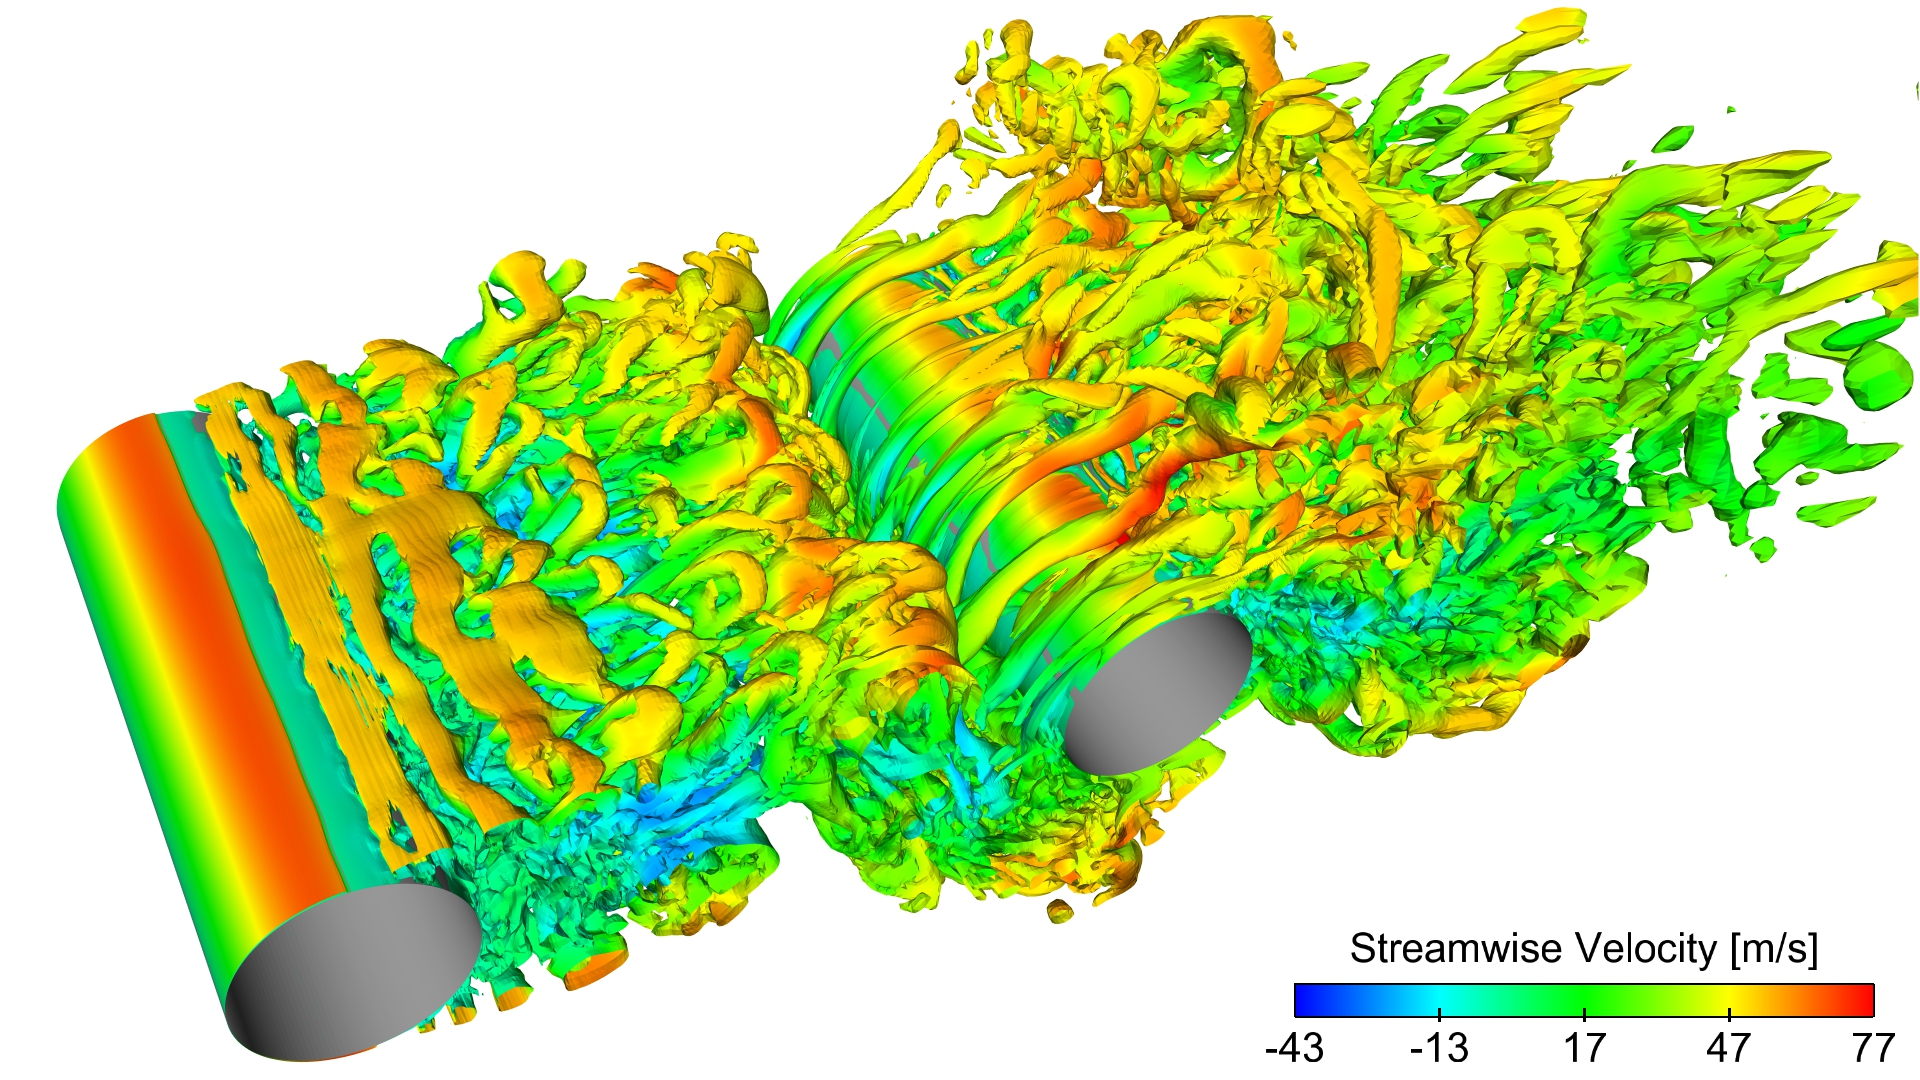
\includegraphics[width=0.40\textwidth]{tc_q_criteria}
    \bicaption{Q判据等值面图,同时测试一下一个很长的标题,比如这真的是一个很长很长很长很长很长很长很长很长的标题. }{Isocontour of Q criteria, at the same time, this is to test a long title, for instance, this is a really very long very long very long very long very long title.}
    \label{fig:tc_q_criteria}
\end{figure}

如果插图的空白区域过大,以图片\verb|shock_cyn|为例,自动裁剪如图\ref{fig:shock_cyn}. 
\begin{figure}[!htbp]
    \centering
    %trim option's parameter order: left bottom right top
    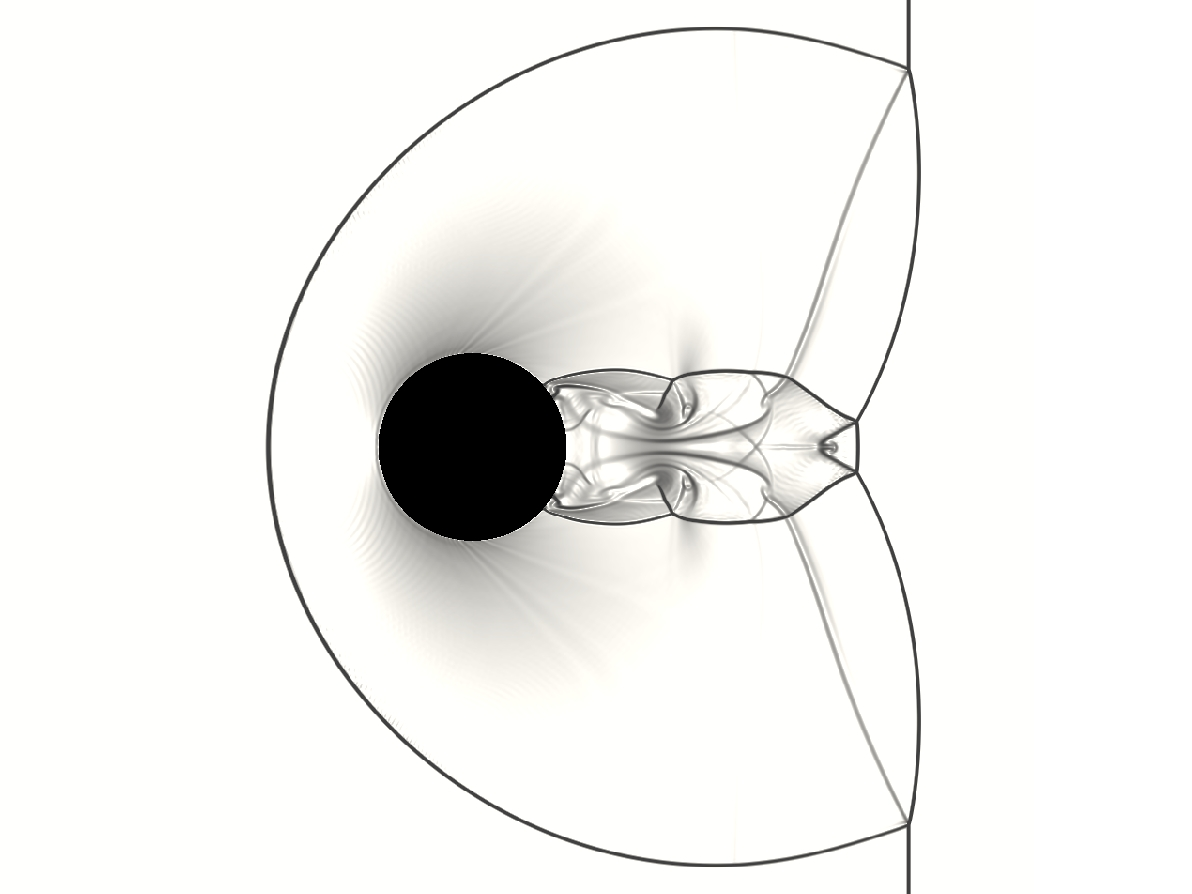
\includegraphics[trim = 30mm 0mm 30mm 0mm, clip, width=0.40\textwidth]{shock_cyn}
    \bicaption{激波圆柱作用. }{Shock-cylinder interaction.}
    \label{fig:shock_cyn}
\end{figure}

多图的插入如图\ref{fig:oaspl},多图不应在子图中给文本子标题,只要给序号,并在主标题中进行引用说明. 
\begin{figure}[!htbp]
    \centering
    \begin{subfigure}[b]{0.35\textwidth}
      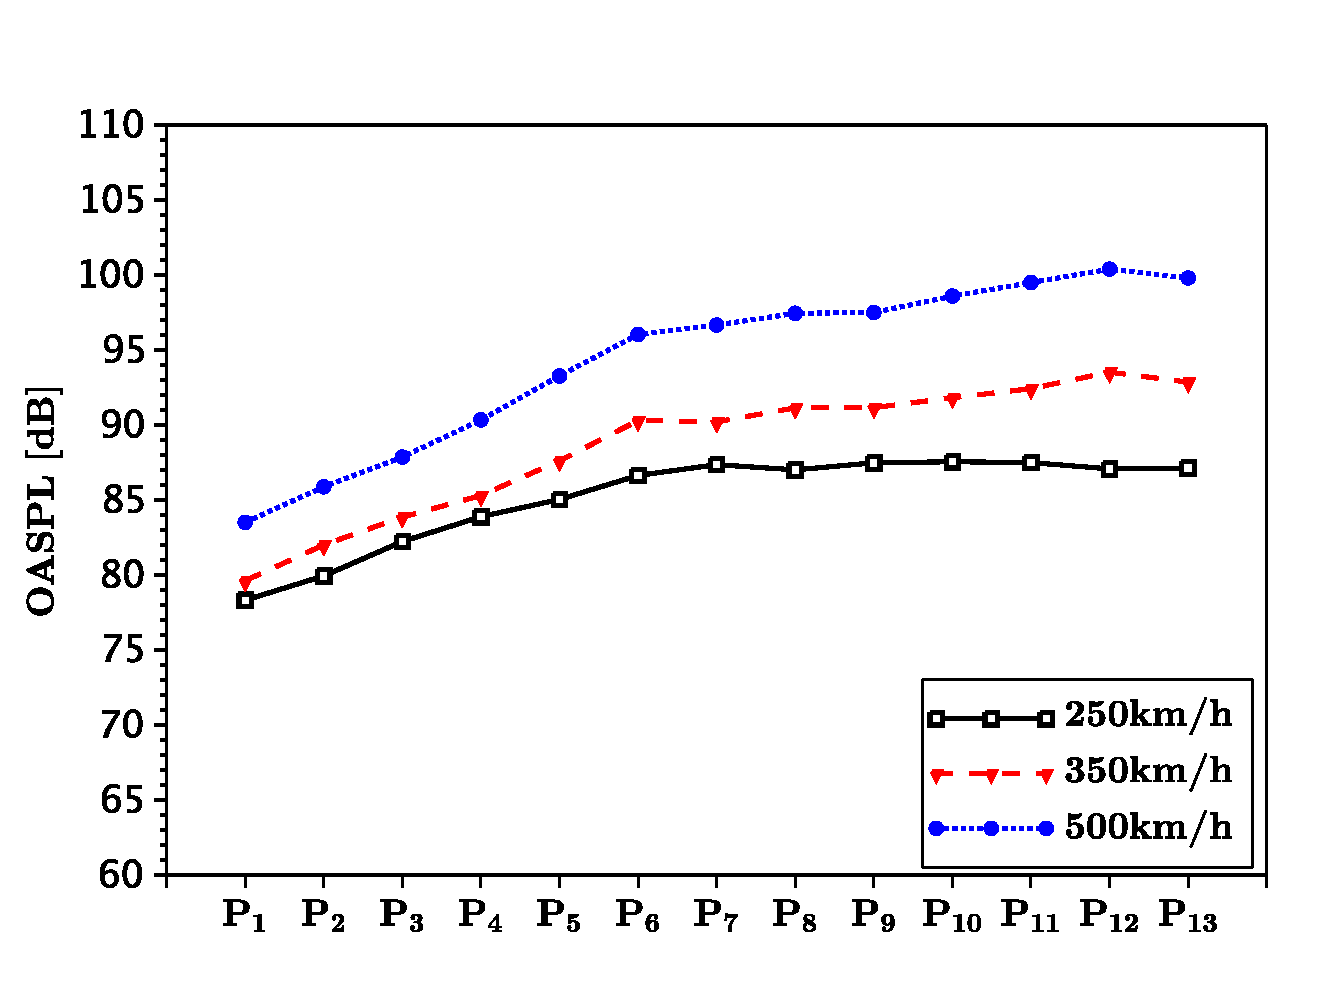
\includegraphics[width=\textwidth]{oaspl_a}
      \caption{}
      \label{fig:oaspl_a}
    \end{subfigure}%
    ~%add desired spacing
    \begin{subfigure}[b]{0.35\textwidth}
      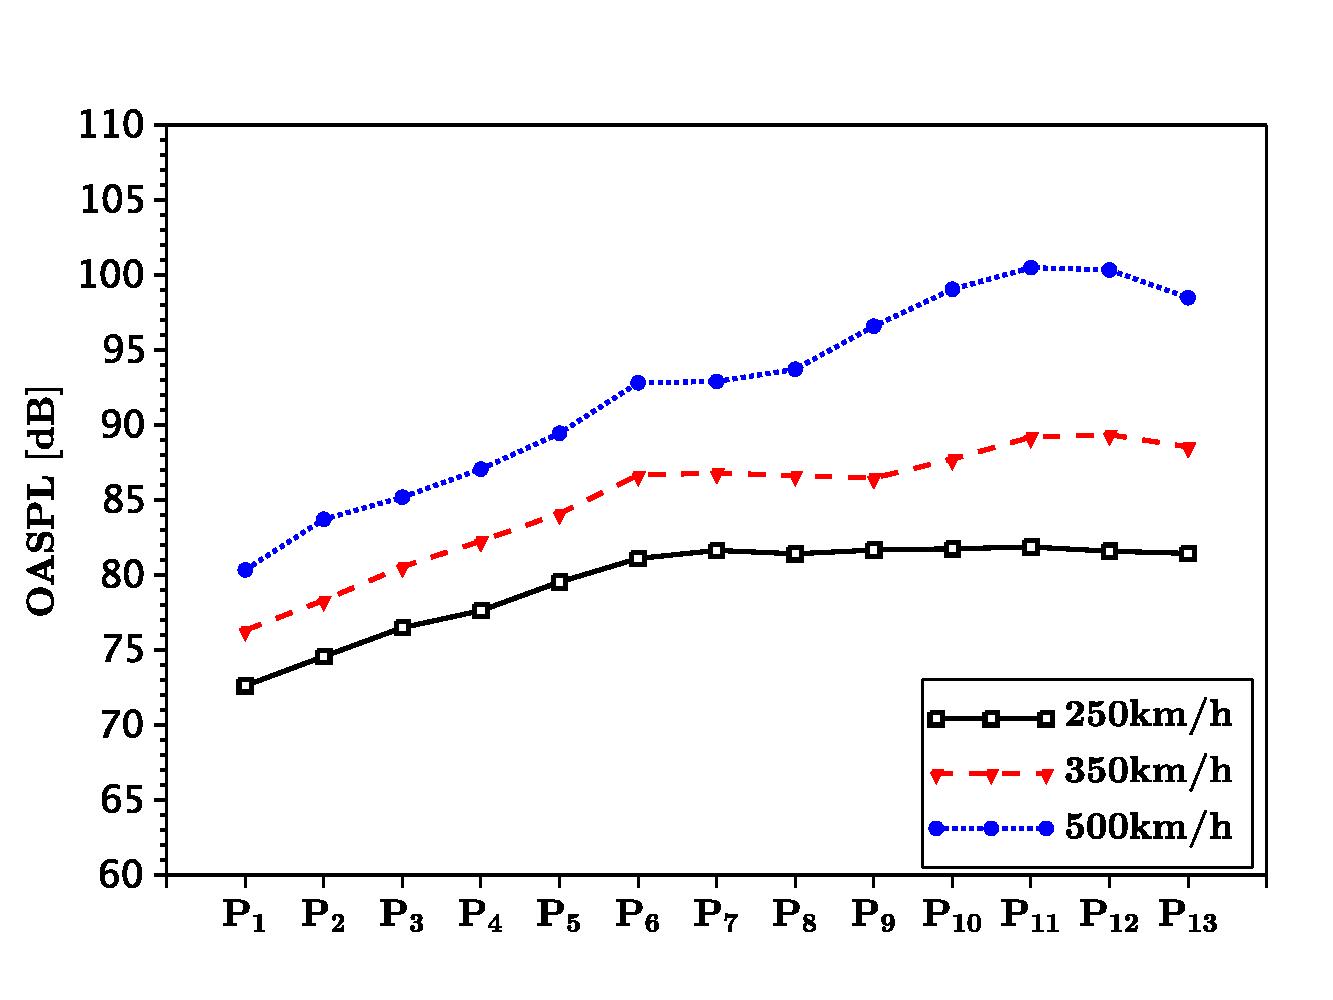
\includegraphics[width=\textwidth]{oaspl_b}
      \caption{}
      \label{fig:oaspl_b}
    \end{subfigure}
    \begin{subfigure}[b]{0.35\textwidth}
      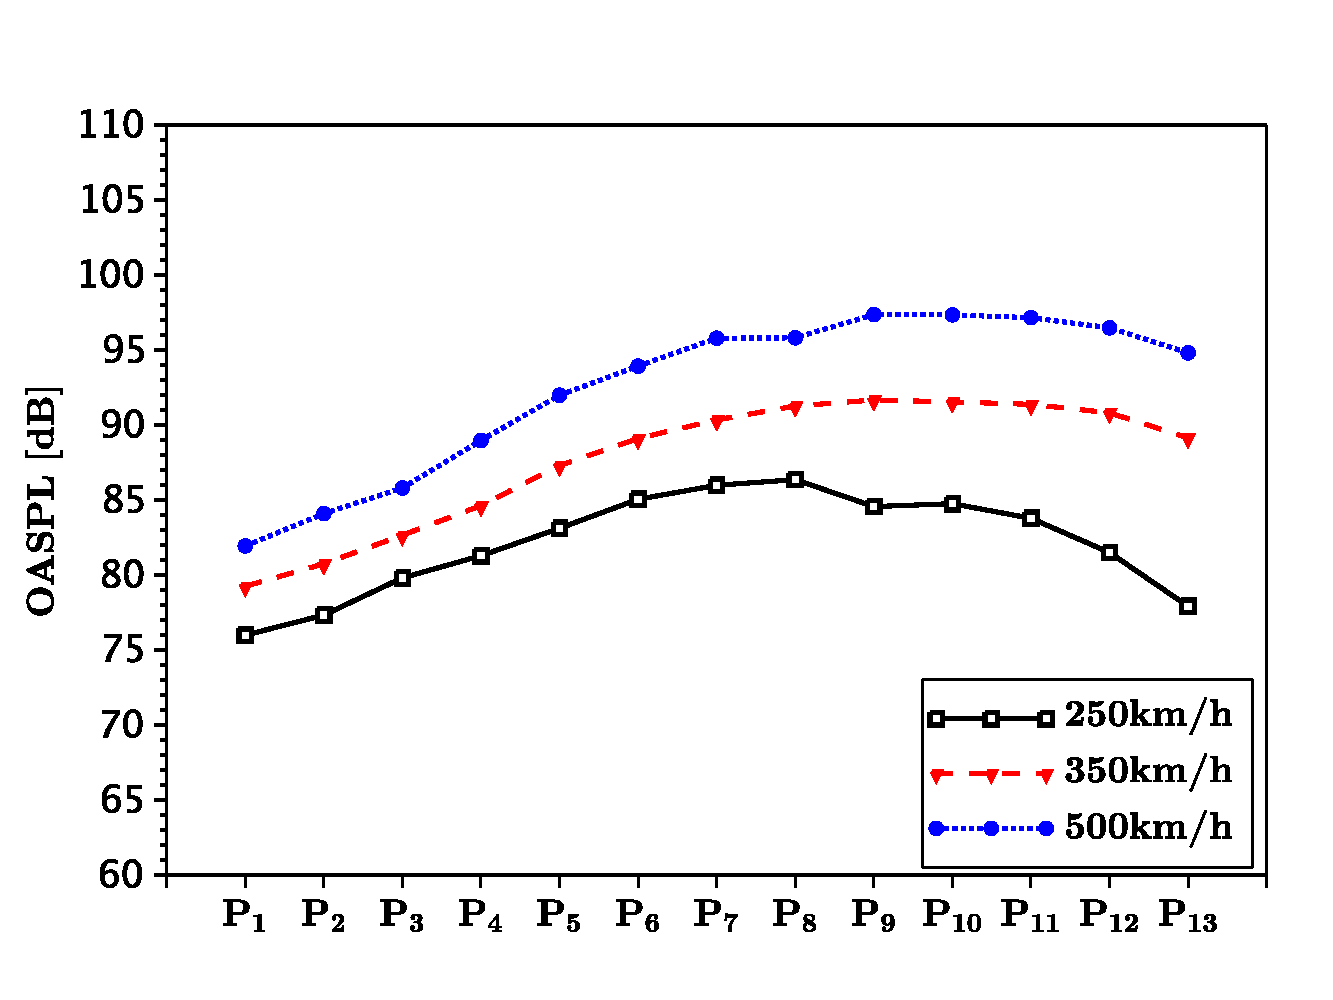
\includegraphics[width=\textwidth]{oaspl_c}
      \caption{}
      \label{fig:oaspl_c}
    \end{subfigure}%
    ~%add desired spacing
    \begin{subfigure}[b]{0.35\textwidth}
      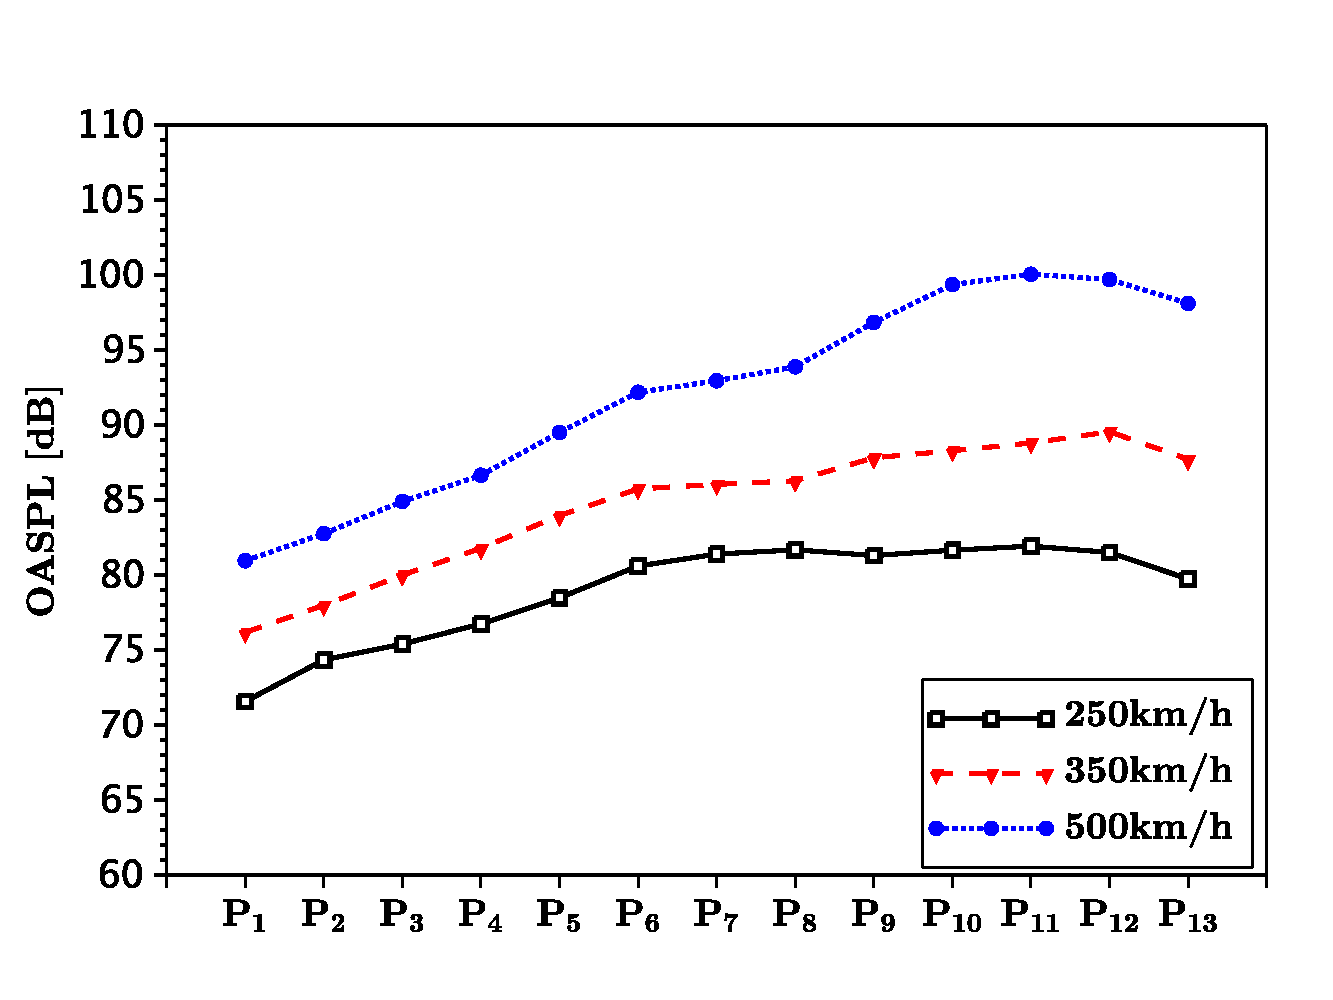
\includegraphics[width=\textwidth]{oaspl_d}
      \caption{}
      \label{fig:oaspl_d}
    \end{subfigure}
    \bicaption{总声压级. (a) 这是子图说明信息,(b) 这是子图说明信息,(c) 这是子图说明信息,(d) 这是子图说明信息. }{OASPL.(a) This is the explanation of subfig, (b) This is the explanation of subfig, (c) This is the explanation of subfig, (d) This is the explanation of subfig.}
    \label{fig:oaspl}
\end{figure}

\subsection{算法}

如见算法~\ref{alg:euclid},详细使用方法请参见文档 \href{https://ctan.org/pkg/algorithmicx?lang=en}{algorithmicx}. 

\begin{algorithm}[!htbp]
    \small
    \caption{Euclid's algorithm}\label{alg:euclid}
    \begin{algorithmic}[1]
        \Procedure{Euclid}{$a,b$}\Comment{The g.c.d. of a and b}
        \State $r\gets a\bmod b$
        \While{$r\not=0$}\Comment{We have the answer if r is 0}
        \State $a\gets b$
        \State $b\gets r$
        \State $r\gets a\bmod b$
        \EndWhile\label{euclidendwhile}
        \State \textbf{return} $b$\Comment{The gcd is b}
        \EndProcedure
    \end{algorithmic}
\end{algorithm}

\subsection{参考文献引用}
%\bibliography{./Biblio/ref}

参考文献引用过程以实例进行介绍,假设需要引用名为"Document Preparation System"的文献,步骤如下:

1)使用Google Scholar搜索Document Preparation System,在目标条目下点击Cite,展开后选择Import into BibTeX打开此文章的BibTeX索引信息,将它们copy添加到ref.bib文件中(此文件位于Biblio文件夹下). 

2)索引第一行 \verb|@article{lamport1986document,|中 \verb|lamport1986document| 即为此文献的label (\textbf{中文文献也必须使用英文label},一般遵照:姓氏拼音+年份+标题第一字拼音的格式),想要在论文中索引此文献,有两种索引类型:

文本类型:\verb|\citet{lamport1986document}|. 正如此处所示 \citet{lamport1986document}; 

括号类型:\verb|\citep{lamport1986document}|. 正如此处所示 \citep{lamport1986document}. 

\textbf{多文献索引用英文逗号隔开}:

\verb|\citep{lamport1986document, chu2004tushu, chen2005zhulu}|. 正如此处所示 \citep{lamport1986document, chu2004tushu, chen2005zhulu}

更多例子如:

\citet{walls2013drought}根据...的研究,首次提出.... 其中关于...\citep{walls2013drought},是当前中国...得到迅速发展的研究领域\citep{chen1980zhongguo}. 引用同一著者在同一年份出版的多篇文献时,在出版年份之后用
英文小写字母区别,如:\citep{yuan2012lana, yuan2012lanb, yuan2012lanc}. 同一处引用多篇文献时,按出版年份由近及远依次标注,中间用
分号分开. 例如\citep{chen1980zhongguo, stamerjohanns2009mathml, hls2012jinji, niu2013zonghe}. 

使用著者-出版年制(authoryear)式参考文献样式时,中文文献必须在BibTeX索引信息的 \textbf{key} 域(请参考ref.bib文件)填写作者姓名的拼音,才能使得文献列表按照拼音排序. 参考文献表中的条目(不排序号),先按语种分类排列,语种顺 序是:中文、日文、英文、俄文、其他文种. 然后,中文按汉语拼音字母顺序排列,日文按第一著者的姓氏笔画排序,西文和 俄文按第一著者姓氏首字母顺序排列. 如中\citep{niu2013zonghe}、日\citep{Bohan1928}、英\citep{stamerjohanns2009mathml}、俄\citep{Dubrovin1906}. 

如此,即完成了文献的索引,请查看下本文档的参考文献一章,看看是不是就是这么简单呢?是的,就是这么简单!

不同文献样式和引用样式,如著者-出版年制(authoryear)、顺序编码制(numbers)、上标顺序编码制(super)可在Thesis.tex中对artratex.sty调用实现,如:
\begin{itemize}
    \footnotesize
    \item \verb+\usepackage[numbers]{artratex}+ $\%$ 文本: Jones [1]; 括号: [1]
    \item \verb+\usepackage[super]{artratex}+ $\%$ 文本: Jones 上标[1]; 括号: 上标[1]
    \item \verb+\usepackage[authoryear]{artratex}+ $\%$ 文本: Jones (1995); 括号: (Jones, 1995)
    \item \verb+\usepackage[alpha]{artratex}+ $\%$ 文本: 不可用; 括号: [Jon95]
\end{itemize}

当前文档的默认参考文献样式为\textbf{authoryear}. 若在上标(\textbf{super})模式下,希望在特定位置将上标改为嵌入式标,可使用

文本类型:\verb|\citetns{lamport1986document,chen2005zhulu}|. 

正如此处所示\citetns{lamport1986document,chen2005zhulu}

括号类型:\verb|\citepns{lamport1986document,chen2005zhulu}|. 

正如此处所示\citepns{lamport1986document,chen2005zhulu}

参考文献索引更为详细的信息,请见 \href{https://github.com/zepinglee/gbt7714-bibtex-style}{zepinglee} 和 \href{https://en.wikibooks.org/wiki/LaTeX/Bibliography_Management}{WiKibook Bibliography}. 

\nocite{*}

\section{常见使用问题}\label{sec:qa}

\begin{enumerate}
    \item 模板每次发布前,都已在Windows,Linux,MacOS系统上测试通过. 下载模板后,若编译出现错误,则请见 \href{https://github.com/mohuangrui/ucasthesis/wiki}{ucasthesis和\LaTeX{}知识小站} 的 \href{https://github.com/mohuangrui/ucasthesis/wiki/%E7%BC%96%E8%AF%91%E6%8C%87%E5%8D%97}{编译指南}. 

    \item 模板文档的编码为UTF-8编码. 所有文件都必须采用UTF-8编码,否则编译后生成的文档将出现乱码文本. 若出现文本编辑器无法打开文档或打开文档乱码的问题,请检查编辑器对UTF-8编码的支持. 如果使用WinEdt作为文本编辑器(\textbf{不推荐使用}),应在其Options -> Preferences -> wrapping选项卡下将两种Wrapping Modes中的内容:
        
        TeX;HTML;ANSI;ASCII|DTX...
        
        修改为:TeX;\textbf{UTF-8|ACP;}HTML;ANSI;ASCII|DTX...
        
        同时,取消Options -> Preferences -> Unicode中的Enable ANSI Format. 

    \item 推荐选择xelatex或lualatex编译引擎编译中文文档. 编译脚本的默认设定为xelatex编译引擎. 你也可以选择不使用脚本编译,如直接使用 \LaTeX{}文本编辑器编译. 注:\LaTeX{}文本编辑器编译的默认设定为pdflatex编译引擎,若选择xelatex或lualatex编译引擎,请进入下拉菜单选择. 为正确生成引用链接,需要进行全编译. 

    \item Texmaker使用简介
        \begin{enumerate}
            \footnotesize
            \item 使用 Texmaker “打开 (Open)” Thesis.tex. 
            \item 菜单 “选项 (Options)” -> “设置当前文档为主文档 (Define as Master Document)”
            \item 菜单 “自定义 (User)” -> “自定义命令 (User Commands)” -> “编辑自定义命令 (Edit User Commands)” -> 左侧选择 “command 1”,右侧 “菜单项 (Menu Item)” 填入 Auto Build -> 点击下方“向导 (Wizard)” -> “添加 (Add)”: xelatex + bibtex + xelatex + xelatex + pdf viewer -> 点击“完成 (OK)”
            \item 使用 Auto Build 编译带有未生成引用链接的源文件,可以仅使用 xelatex 编译带有已经正确生成引用链接的源文件. 
            \item 编译完成,“查看(View)” PDF,在PDF中 “ctrl+click” 可链接到相对应的源文件. 
        \end{enumerate}
    
    \item 模版的设计可能地考虑了适应性. 致谢等所有条目都是通过最为通用的

        \verb+\chapter{item name}+  and \verb+\section*{item name}+

        来显式实现的 (请观察Backmatter.tex),从而可以随意添加,放置,和修改,如同一般章节. 对于图表目录名称则可在ucasthesis.cfg中进行修改. 

    \item 设置文档样式: 在artratex.sty中搜索关键字定位相应命令,然后修改
        \begin{enumerate}
            \item 正文行距:启用和设置 \verb|\linespread{1.5}|,默认1.5倍行距. 
            \item 参考文献行距:修改 \verb|\setlength{\bibsep}{0.0ex}|
            \item 目录显示级数:修改 \verb|\setcounter{tocdepth}{2}|
            \item 文档超链接的颜色及其显示:修改 \verb|\hypersetup|
        \end{enumerate}

    \item 文档内字体切换方法:
        \begin{itemize}
            \item 宋体:国科大论文模板ucasthesis 或 \textrm{国科大论文模板ucasthesis}
            \item 粗宋体:{\bfseries 国科大论文模板ucasthesis} 或 \textbf{国科大论文模板ucasthesis}
            \item 黑体:{\sffamily 国科大论文模板ucasthesis} 或 \textsf{国科大论文模板ucasthesis}
            \item 粗黑体:{\bfseries\sffamily 国科大论文模板ucasthesis} 或 \textsf{\bfseries 国科大论文模板ucasthesis}
            \item 仿宋:{\ttfamily 国科大论文模板ucasthesis} 或 \texttt{国科大论文模板ucasthesis}
            \item 粗仿宋:{\bfseries\ttfamily 国科大论文模板ucasthesis} 或 \texttt{\bfseries 国科大论文模板ucasthesis}
            \item 楷体:{\itshape 国科大论文模板ucasthesis} 或 \textit{国科大论文模板ucasthesis}
            \item 粗楷体:{\bfseries\itshape 国科大论文模板ucasthesis} 或 \textit{\bfseries 国科大论文模板ucasthesis}
        \end{itemize}

    \item 封面下划线上的文本不居中下划线,这是因为下划线前面还有字头,导致文本只能在页面居中和在下划线上居中二选一. 当前封面采取页面居中. 如需要调整文本在下划线上的位置,可用 \verb|\hspace{+/- n.0em}| 命令来插入或删除 n 个空格,进行手动调整,比如

        \verb|\advisor{\hspace{+3.0em} xxx~研究员~xxx单位}|
                
    有时下划线看上去粗细不一致,这是显示的问题,打印正常. 
\end{enumerate}



%---------------------------------------------------------------------------%
% main content
	%-
	%-> Appendix
	%-
	\cleardoublepage%
	\appendix% initialize the environment
	\chapter{中国科学院大学学位论文撰写要求}

学位论文是研究生科研工作成果的集中体现,是评判学位申请者学术水平、授予其学位的主要依据,是科研领域重要的文献资料。根据《科学技术报告、学位论文和学术论文的编写格式》(GB/T 7713-1987)、《学位论文编写规则》(GB/T 7713.1-2006)和《文后参考文献著录规则》(GB7714—87)等国家有关标准,结合中国科学院大学(以下简称“国科大”)的实际情况,特制订本规定。

\section{论文无附录者无需附录部分}

\section{测试公式编号} \label{sec:testmath}

\begin{equation} \label{eq:appedns}
    \begin{cases}
        \frac{\partial \rho}{\partial t} + \nabla\cdot(\rho\Vector{V}) = 0 \ \mathrm{times\ font\ test}\\
        \frac{\partial (\rho\Vector{V})}{\partial t} + \nabla\cdot(\rho\Vector{V}\Vector{V}) = \nabla\cdot\Tensor{\sigma} \ \text{times font test}\\
        \frac{\partial (\rho E)}{\partial t} + \nabla\cdot(\rho E\Vector{V}) = \nabla\cdot(k\nabla T) + \nabla\cdot(\Tensor{\sigma}\cdot\Vector{V})
    \end{cases}
\end{equation}
\begin{equation}
    \frac{\partial }{\partial t}\int\limits_{\Omega} u \, \mathrm{d}\Omega + \int\limits_{S} \unitVector{n}\cdot(u\Vector{V}) \, \mathrm{d}S = \dot{\phi}
\end{equation}

\section{测试生僻字}

霜蟾盥薇曜灵霜颸妙鬘虚霩淩澌菀枯菡萏泬寥窅冥毰毸濩落霅霅便嬛岧峣瀺灂姽婳愔嫕飒纚棽俪緸冤莩甲摛藻卮言倥侗椒觞期颐夜阑彬蔚倥偬澄廓簪缨陟遐迤逦缥缃鹣鲽憯懔闺闼璀错媕婀噌吰澒洞阛闠覼缕玓瓑逡巡諓諓琭琭瀌瀌踽踽叆叇氤氲瓠犀流眄蹀躞赟嬛茕頔璎珞螓首蘅皋惏悷缱绻昶皴皱颟顸愀然菡萏卑陬纯懿犇麤掱暒 墌墍墎墏墐墒墒墓墔墕墖墘墖墚墛坠墝增墠墡墢墣墤墥墦墧墨墩墪樽墬墭堕墯墰墱墲坟墴墵垯墷墸墹墺墙墼墽垦墿壀壁壂壃壄壅壆坛壈壉壊垱壌壍埙壏壐壑壒压壔壕壖壗垒圹垆壛壜壝垄壠壡坜壣壤壥壦壧壨坝塆圭嫶嫷嫸嫹嫺娴嫼嫽嫾婳妫嬁嬂嬃嬄嬅嬆嬇娆嬉嬊娇嬍嬎嬏嬐嬑嬒嬓嬔嬕嬖嬗嬘嫱嬚嬛嬜嬞嬟嬠嫒嬢嬣嬥嬦嬧嬨嬩嫔嬫嬬奶嬬嬮嬯婴嬱嬲嬳嬴嬵嬶嬷婶嬹嬺嬻嬼嬽嬾嬿孀孁孂娘孄孅孆孇孆孈孉孊娈孋孊孍孎孏嫫婿媚嵭嵮嵯嵰嵱嵲嵳嵴嵵嵶嵷嵸嵹嵺嵻嵼嵽嵾嵿嶀嵝嶂嶃崭嶅嶆岖嶈嶉嶊嶋嶌嶍嶎嶏嶐嶑嶒嶓嵚嶕嶖嶘嶙嶚嶛嶜嶝嶞嶟峤嶡峣嶣嶤嶥嶦峄峃嶩嶪嶫嶬嶭崄嶯嶰嶱嶲嶳岙嶵嶶嶷嵘嶹岭嶻屿岳帋巀巁巂巃巄巅巆巇巈巉巊岿巌巍巎巏巐巑峦巓巅巕岩巗巘巙巚帠帡帢帣帤帨帩帪帬帯帰帱帲帴帵帷帹帺帻帼帽帾帿幁幂帏幄幅幆幇幈幉幊幋幌幍幎幏幐幑幒幓幖幙幚幛幜幝幞帜幠幡幢幤幥幦幧幨幩幪幭幮幯幰幱庍庎庑庖庘庛庝庠庡庢庣庤庥庨庩庪庬庮庯庰庱庲庳庴庵庹庺庻庼庽庿廀厕廃厩廅廆廇廋廌廍庼廏廐廑廒廔廕廖廗廘廙廛廜廞庑廤廥廦廧廨廭廮廯廰痈廲廵廸廹廻廼廽廿弁弅弆弇弉弖弙弚弜弝弞弡弢弣弤弨弩弪弫弬弭弮弰弲弪弴弶弸弻弼弽弿彖彗彘彚彛彜彝彞彟彴彵彶彷彸役彺彻彽彾佛徂徃徆徇徉后徍徎徏径徒従徔徕徖徙徚徛徜徝从徟徕御徢徣徤徥徦徧徨复循徫旁徭微徯徰徱徲徳徴徵徶德徸彻徺忁忂惔愔忇忈忉忔忕忖忚忛応忝忞忟忪挣挦挧挨挩挪挫挬挭挮挰掇授掉掊掋掍掎掐掑排掓掔掕挜掚挂掜掝掞掟掠采探掣掤掦措掫掬掭掮掯掰掱掲掳掴掵掶掸掹掺掻掼掽掾掿拣揁揂揃揅揄揆揇揈揉揊揋揌揍揎揑揓揔揕揖揗揘揙揤揥揦揧揨揫捂揰揱揲揳援揵揶揷揸揻揼揾揿搀搁搂搃搄搅搇搈搉搊搋搌搎搏搐搑搒摓摔摕摖摗摙摚摛掼摝摞摠摡斫斩斮斱斲斳斴斵斶斸旪旫旮旯晒晓晔晕晖晗晘晙晛晜晞晟晠晡晰晣晤晥晦晧晪晫晬晭晰晱晲晳晴晵晷晸晹晻晼晽晾晿暀暁暂暃暄暅暆暇晕晖暊暋暌暍暎暏暐暑暒暓暔暕暖暗旸暙暚暛暜暝暞暟暠暡暣暤暥暦暧暨暩暪暬暭暮暯暰昵暲暳暴暵暶暷暸暹暺暻暼暽暾暿曀曁曂曃晔曅曈曊曋曌曍曎曏曐曑曒曓曔曕曗曘曙曚曛曜曝曞曟旷曡曢曣曤曥曦曧昽曩曪曫晒曭曮曯椗椘椙椚椛検椝椞椟椠椡椢椣椤椥椦椧椨椩椪椫椬椭椮椯椰椱椲椳椴椵椶椷椸椹椺椻椼椽椾椿楀楁楂楃楅楆楇楈楉杨楋楌楍榴榵榶榷榸榹榺榻榼榽榾桤槀槁槂盘槄槅槆槇槈槉槊构槌枪槎槏槐槑槒杠槔槕槖槗滙滛滜滝滞滟滠滢滣滦滧滪滫沪滭滮滰滱渗滳滵滶滹滺浐滼滽漀漃漄漅漈漉溇漋漌漍漎漐漑澙熹漗漘漙沤漛漜漝漞漟漡漤漥漦漧漨漪渍漭漮漯漰漱漳漴溆漶漷漹漺漻漼漽漾浆潀颍潂潃潄潅潆潇潈潉潊潋潌潍潎潏潐潒潓洁潕潖潗潘沩潚潜潝潞潟潠潡潢潣润潥潦潧潨潩潪潫潬潭浔溃潱潲潳潴潵潶滗潸潹潺潻潼潽潾涠澁澄澃澅浇涝澈澉澊澋澌澍澎澏湃澐澑澒澓澔澕澖涧澘澙澚澛澜澝澞澟渑澢澣泽浍澯澰淀澲澳澴澵澶澷澸潇潆瀡瀢瀣瀤瀥潴泷濑瀩瀪瀫瀬瀭瀮瀯弥瀱潋瀳瀴瀵瀶瀷瀸瀹瀺瀻瀼瀽澜瀿灀灁瀺灂沣滠灅灆灇灈灉灊灋灌灍灎灏灐洒灒灓漓灖灗滩灙灚灛灜灏灞灟灠灡灢湾滦灥灦灧灨灪燝燞燠燡燢燣燤燥灿燧燨燩燪燫燮燯燰燱燲燳烩燵燵燸燹燺薰燽焘燿爀爁爂爃爄爅爇爈爉爊爋爌烁爎爏爑爒爓爔爕爖爗爘爙爚烂爜爝爞爟爠爡爢爣爤爥爦爧爨爩猽猾獀犸獂獆獇獈獉獊獋獌獍獏獐獑獒獓獔獕獖獗獘獙獚獛獜獝獞獟獠獡獢獣獤獥獦獧獩狯猃獬獭狝獯狞獱獳獴獶獹獽獾獿猡玁玂玃。
% appendix content
	%-
	%-> Backmatter: bibliography, glossary, index
	%-
	\backmatter% initialize the environment
	\intotoc{\bibname}% add link to contents table and bookmark
	\bibliography{Biblio/ref}% bibliography
	%\chapter{作者简历及攻读学位期间发表的学术论文与研究成果}
%
%\textbf{本科生无需此部分}。
%
%\section*{作者简历}
%
%\subsection*{casthesis作者}
%
%吴凌云,福建省屏南县人,中国科学院数学与系统科学研究院博士研究生。
%
%\subsection*{ucasthesis作者}
%
%莫晃锐,湖南省湘潭县人,中国科学院力学研究所硕士研究生。
%
%\section*{已发表(或正式接受)的学术论文:}
%
%[1] ucasthesis: A LaTeX Thesis Template for the University of Chinese Academy of Sciences, 2014.
%
%\section*{申请或已获得的专利:}
%
%(无专利时此项不必列出)
%
%\section*{参加的研究项目及获奖情况:}
%
%可以随意添加新的条目或是结构。

\chapter[致谢]{致\quad 谢}\chaptermark{致\quad 谢}% syntax: \chapter[目录]{标题}\chaptermark{页眉}
%\thispagestyle{noheaderstyle}% 如果需要移除当前页的页眉
%\pagestyle{noheaderstyle}% 如果需要移除整章的页眉
\pagestyle{mainmatterstyle} % 与前文页眉页脚格式相同

感激casthesis作者吴凌云学长,gbt7714-bibtex-style
开发者zepinglee,和ctex众多开发者们。若没有他们的辛勤付出和非凡工作,\LaTeX{}菜鸟的我是无法完成此国科大学位论文\LaTeX{}模板ucasthesis的。在\LaTeX{}中的一点一滴的成长源于开源社区的众多优秀资料和教程,在此对所有\LaTeX{}社区的贡献者表示感谢!

ucasthesis国科大学位论文\LaTeX{}模板的最终成型离不开以霍明虹老师和丁云云老师为代表的国科大学位办公室老师们制定的官方指导文件和众多ucasthesis用户的热心测试和耐心反馈,在此对他们的认真付出表示感谢。特别对国科大的赵永明同学的众多有效反馈意见和建议表示感谢,对国科大本科部的陆晴老师和本科部学位办的丁云云老师的细致审核和建议表示感谢。谢谢大家的共同努力和支持,让ucasthesis为国科大学子使用\LaTeX{}撰写学位论文提供便利和高效这一目标成为可能。

\cleardoublepage[plain]% 让文档总是结束于偶数页,可根据需要设定页眉页脚样式,如 [noheaderstyle]

% other information
\end{document}
%---------------------------------------------------------------------------%

